While LAPACK~\cite{lug99} linear algebra factorization
algorithms were successful in exploiting early cache-based
architectures, they have shown significant performance
limitations on modern many/multi-core architectures and many
well-tuned LAPACK-style kernels
fail to achieve satisfactory performance on these
architectures~\cite{agullo2009comparative}.
As reported by Dongarra et al\@.~in~\cite{dongarra2011achieving},
three factors contribute to this
performance penalty.

The first factor is the fork-join parallelism
model appearing in LAPACK when it is linked with multi-threaded BLAS.
This model induces a high overhead on
massively parallel architectures since it introduces many unnecessary
synchronization points, keeping many computational resources frequently
idle.
Secondly, LAPACK processes data at a coarse granularity,
typically working on the block-column level (also known as a panel),
which fails to exhibit enough parallelism to
keep all the cores busy.
Finally, while all factorization algorithms in LAPACK are based on
a recursive panel factorization followed by an update to the
corresponding trailing matrix,
the panel factorization uses memory-bound operations
(i.e.\ level-1 and level-2 BLAS operations).

In order to use modern many/multi-core architectures at full
efficiency, a new generation of linear algebra libraries such as
PLASMA~\cite{DBLP:journals/corr/abs-0709-1272}
have cast LAPACK panel-based algorithms into tile algorithms. Tile
algorithms enjoy the property of addressing each of the three
drawbacks that keep LAPACK from providing a reasonable performance on
modern massively parallel architectures.
In fact, tile algorithms operate at a
finer granularity by dividing the whole matrix into
small square tiles which are more likely to fit into fast memory,
such as the L2 cache of a CPU, as illustrated in Figure~\ref{fig:tile_algo}.
\begin{figure}[th]
  \captionsetup[subfigure]{justification=justified,singlelinecheck=false}
  \begin{subfigure}[t]{0.3 \textwidth}
    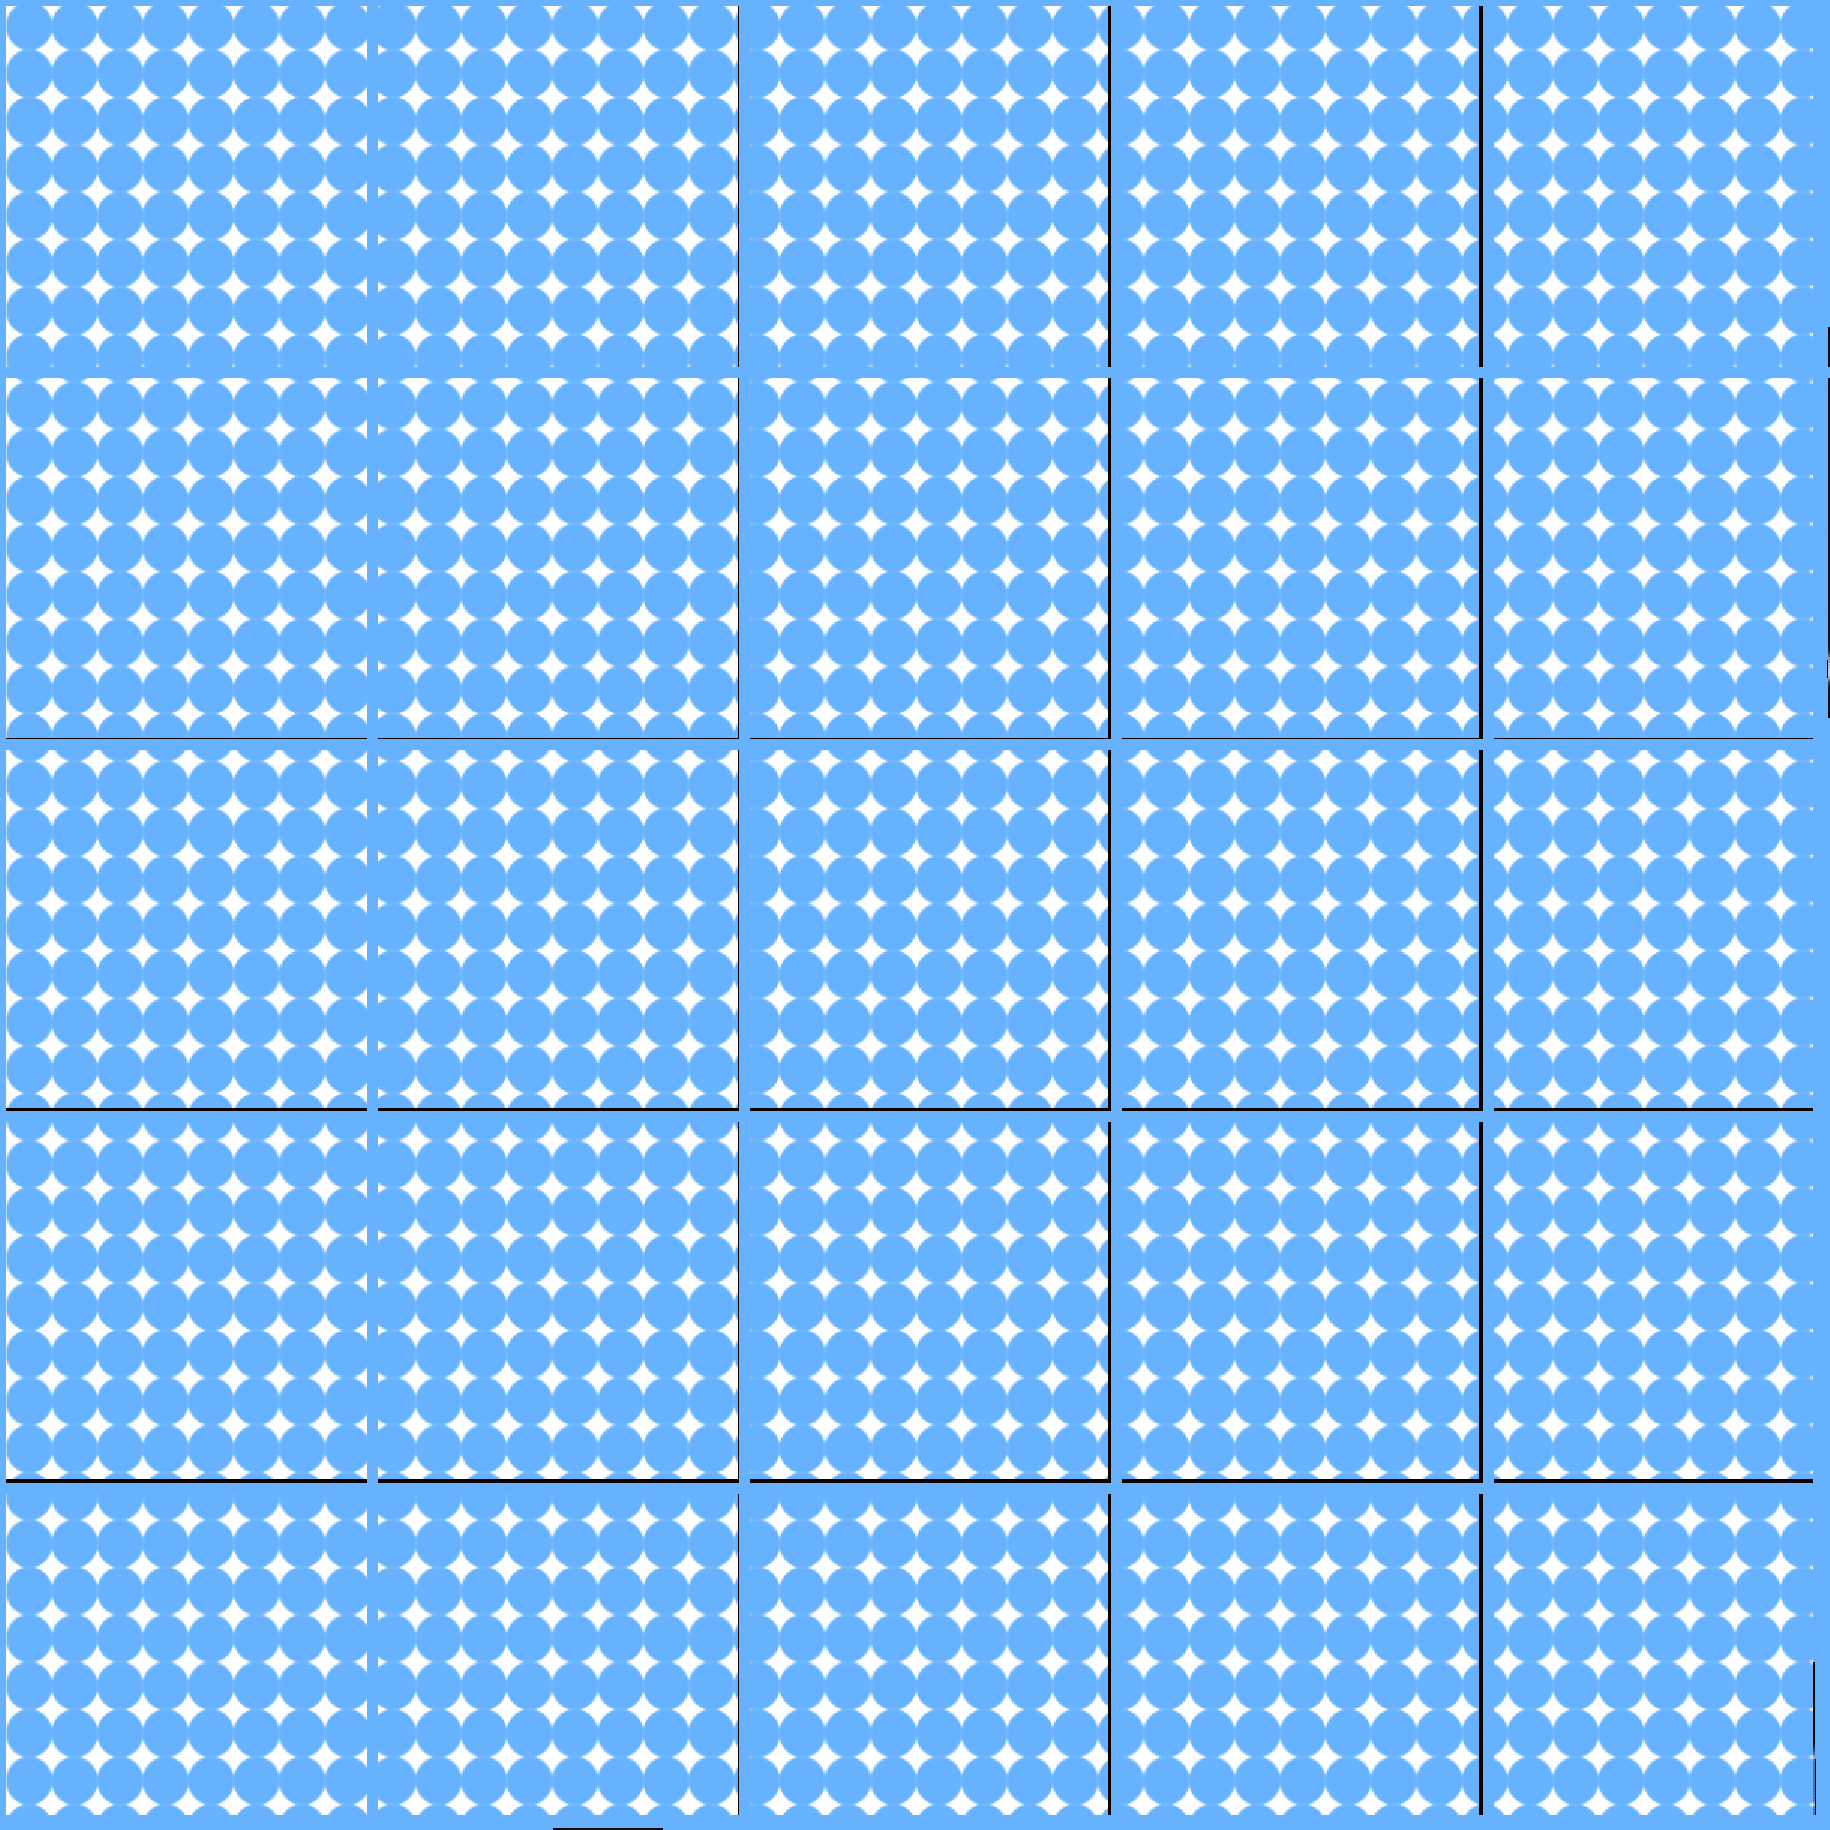
\includegraphics[width=3.5cm, height=3.5cm]{fig/one-sided-initial}
    \caption{\label{fig:initial_matrix}Initial matrix.}
  \end{subfigure}
  \hfill
  \begin{subfigure}[t]{0.3 \textwidth}
    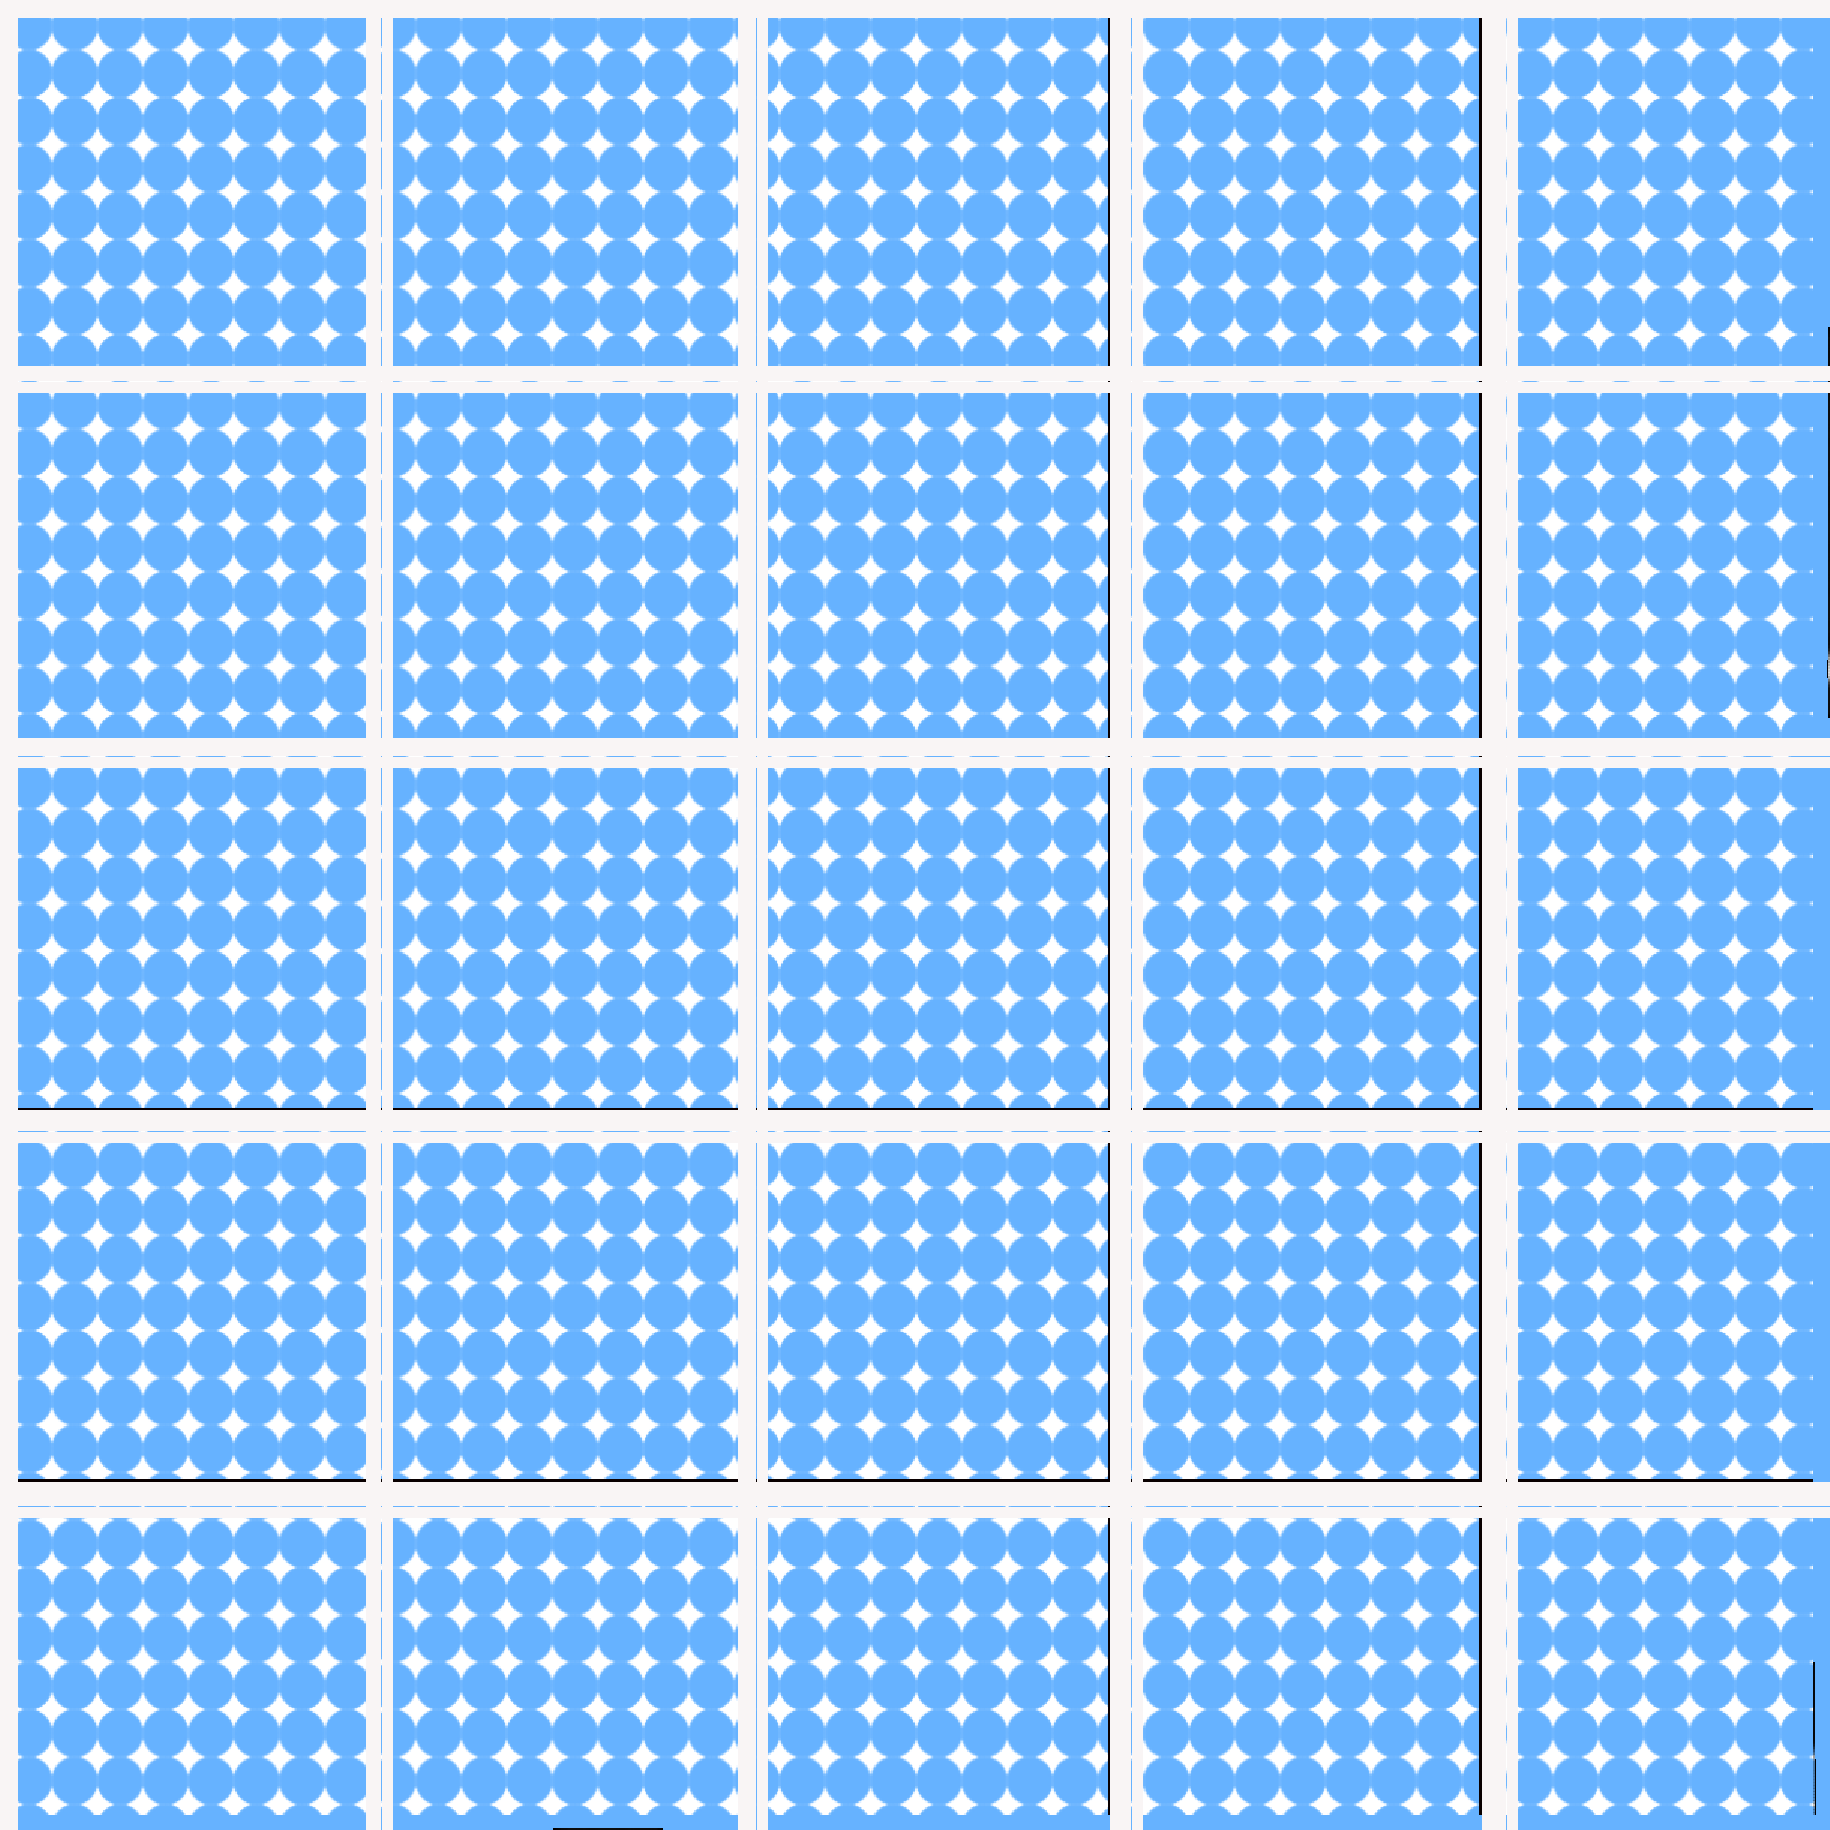
\includegraphics[width=3.5cm, height=3.5cm]{fig/one-sided-tile}
    \caption{\label{fig:tile_matrix}
      $5\times 5$ tile matrix.}
  \end{subfigure}
  \hfill
    \begin{subfigure}[t]{0.3 \textwidth}
    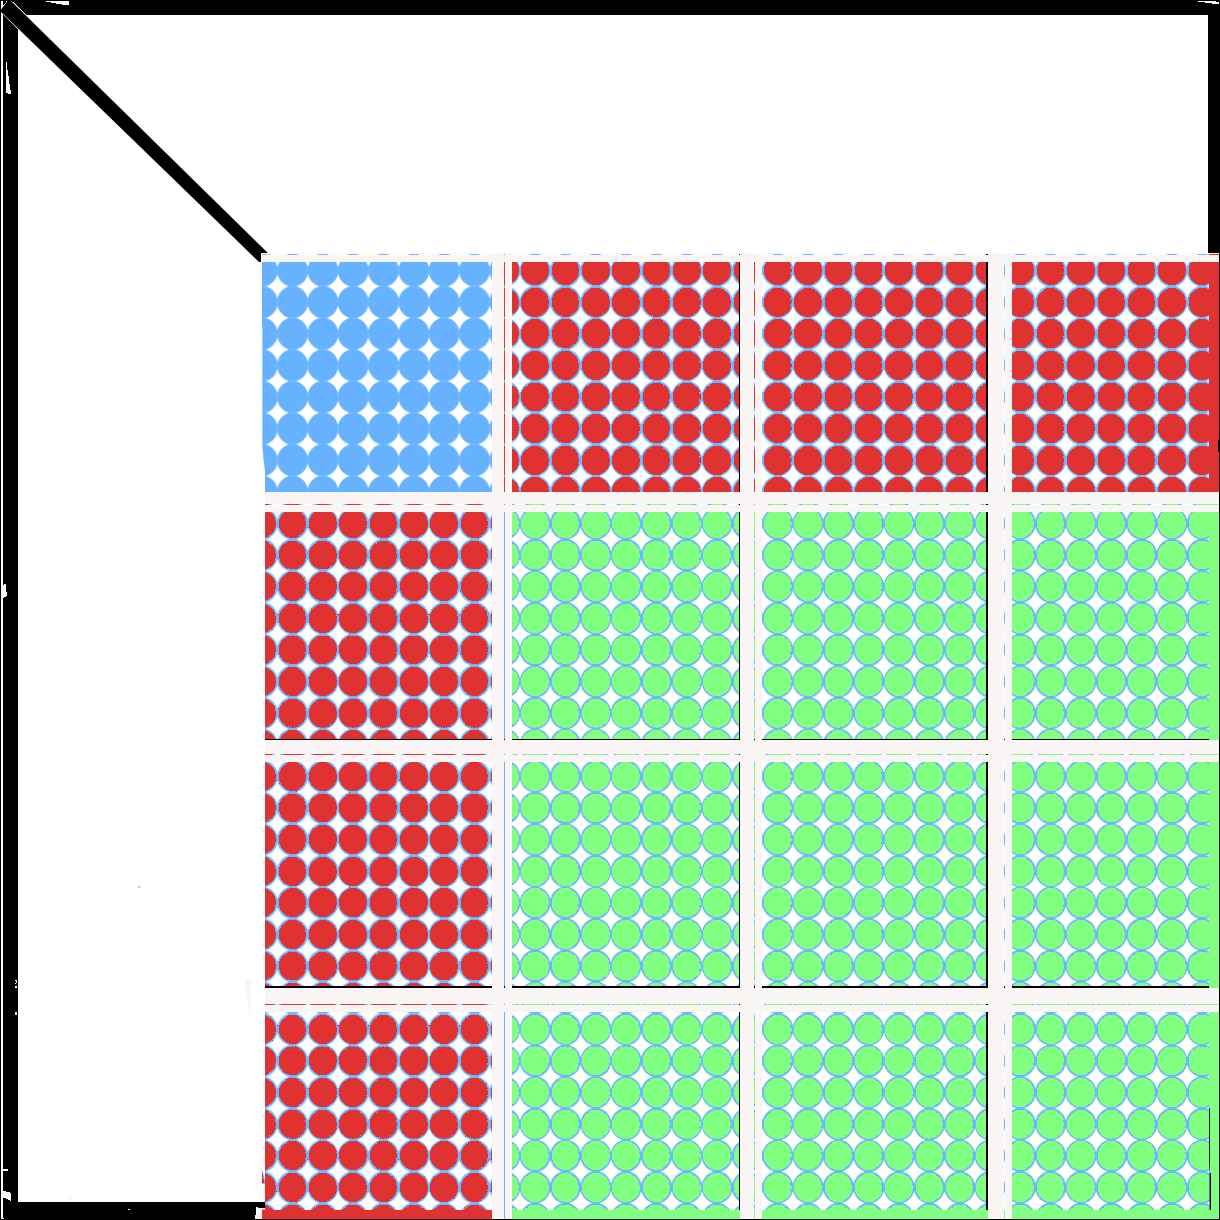
\includegraphics[width=3.5cm, height=3.5cm]{fig/one-sided-tile-facto}
    \caption{\label{fig:tile_facto}
     Many kernels operating on different tiles in parallel.}
  \end{subfigure}
  \caption{Illustration of matrix division in square tiles as is the case
    in tile algorithms. This helps working at  a finer granularity to
    keep the maximum number of cores busy.}
    \label{fig:tile_algo}
\end{figure}

The order of execution of the tasks in tile algorithms are commonly
represented in the form of a DAG in which each node represents a task, while
the edges represent the data dependencies between the tasks.  These
tasks are then scheduled by a runtime system that checks the
dependencies and takes care of launching tasks on appropriate cores.

The superiority of the tile layout algorithms over traditional
approaches has been demonstrated conclusively through a one-sided
factorization benchmark suite~\cite{agullo2009comparative}.

In the last few years,
the PLASMA development team dedicated their full
energy to designing highly efficient tile
algorithms for one-sided factorizations.
In 2008, Buttari et al.~\cite{buttari2008parallel},
introduced the first algorithm for parallel tiled $QR$ factorization for
multicore architectures.
This algorithm was extended in 2010 by
Hadri et al.~\cite{hadri2010tile} to present a new fully asynchronous
method for computing a $QR$ factorization of tall and skinny matrices.
The Cholesky and $LU$ factorization versions are studied
in~\cite{DBLP:journals/corr/abs-0709-1272}, while the algorithm to
compute the $LDL^T$ factorization of symmetric indefinite matrices is
discussed in~\cite{becker2011towards}
(though we add pivoting in the implementations compared here).

This work revisits the state-of-the-art tile algorithms for
one-sided factorizations and provides an
efficient task-based OpenMP implementation for comparison with
other runtime systems.
